\documentclass[11pt,a4paper]{jsarticle}

\usepackage[dvipdfmx]{graphicx}
\usepackage{graphicx}
\usepackage[top=20truemm,bottom=20truemm,left=25truemm,right=25truemm]{geometry}
\usepackage{comment}


\title{ナノ科学レポート (1/11提出分)}
\author{東大物理工学科 03-153012 平松信義}
\date{\today}
\begin{document}
\maketitle

Coulomb islandの電位を$\phi$とおく. 電荷の中性条件から
\begin{eqnarray}
-ne &=& C_g (\phi-V_g)  + C_1(\phi+\frac{V}{2}) + C_2 (\phi-\frac{V}{2}) \nonumber \\
\iff \phi &=& \frac{1}{C_\Sigma} [-ne+C_gV_g +\frac{V}{2} (C_2-C_1)].
\end{eqnarray}
ただし$C_\Sigma=C_g+C_1+C_2$とおいた.

Coulomb islandの静電エネルギー$U(n)$と電気化学ポテンシャル$\mu(n)$はそれぞれ, 
\begin{eqnarray}
U(n) &=& \frac{C_\Sigma}{2}\phi^2, \\
\mu(n) &=& U(n) - U(n-1) \nonumber \\
&=& \frac{e^2}{C_\Sigma} (n-\frac{1}{2}) -  \frac{e}{C_\Sigma} [C_gV_g +\frac{V}{2} (C_2-C_1)].
\end{eqnarray}

一方, キャパシタ$C_1$を挟んでドレイン側の電気化学ポテンシャル$\mu_1$と, キャパシタ$C_2$を挟んでソース側の電気化学ポテンシャル$\mu_2$は, それぞれ, 
\begin{eqnarray}
\mu_1 &=& \frac{eV}{2},\\
\mu_2 &=& -\frac{eV}{2}.
\end{eqnarray}

$n$番目の電子がドレインからキャパシタ$C_1$をまたいでCoulomb islandにトンネルできない条件は,
\begin{eqnarray}
\mu(n) &>& \mu_1, \nonumber \\
\iff V &>& - \frac{2C_g}{2C_1+C_g}V_g +\frac{2n-1}{2C_1+C_g}e.
\end{eqnarray}

同様に、$n-1$番目の電子がCoulomb islandからキャパシタ$C_2$をまたいでソースにトンネルできない条件は, 
\begin{eqnarray}
\mu(n-1) &>& \mu_2, \nonumber \\
\iff V &<&  \frac{2C_g}{2C_2+C_g}V_g -\frac{2n-3}{2C_2+C_g}e.
\end{eqnarray}


(i) $C_1=C_2>>C_g$とする。不等式(6),(7)が成り立ちクーロン閉塞が起こる条件は,
\begin{eqnarray}
-\frac{C_g}{C_2}V_g -\frac{2n-1}{2C_2}e< V <  \frac{C_g}{C_2}V_g -\frac{2n-3}{2C_2}e.
\end{eqnarray}
図1にクーロン閉塞により電流が流れなくなる領域を示す。

(ii) $C_1=4C_2>>C_g$とする. クーロン閉塞が起こる条件は,
\begin{eqnarray}
-\frac{C_g}{4C_2}V_g -\frac{2n-1}{8C_2}e< V <  \frac{C_g}{C_2}V_g -\frac{2n-3}{2C_2}e.
\end{eqnarray}
図2にクーロン閉塞により電流が流れなくなる領域を示す。

\begin{figure}[htb]
    \begin{center}
   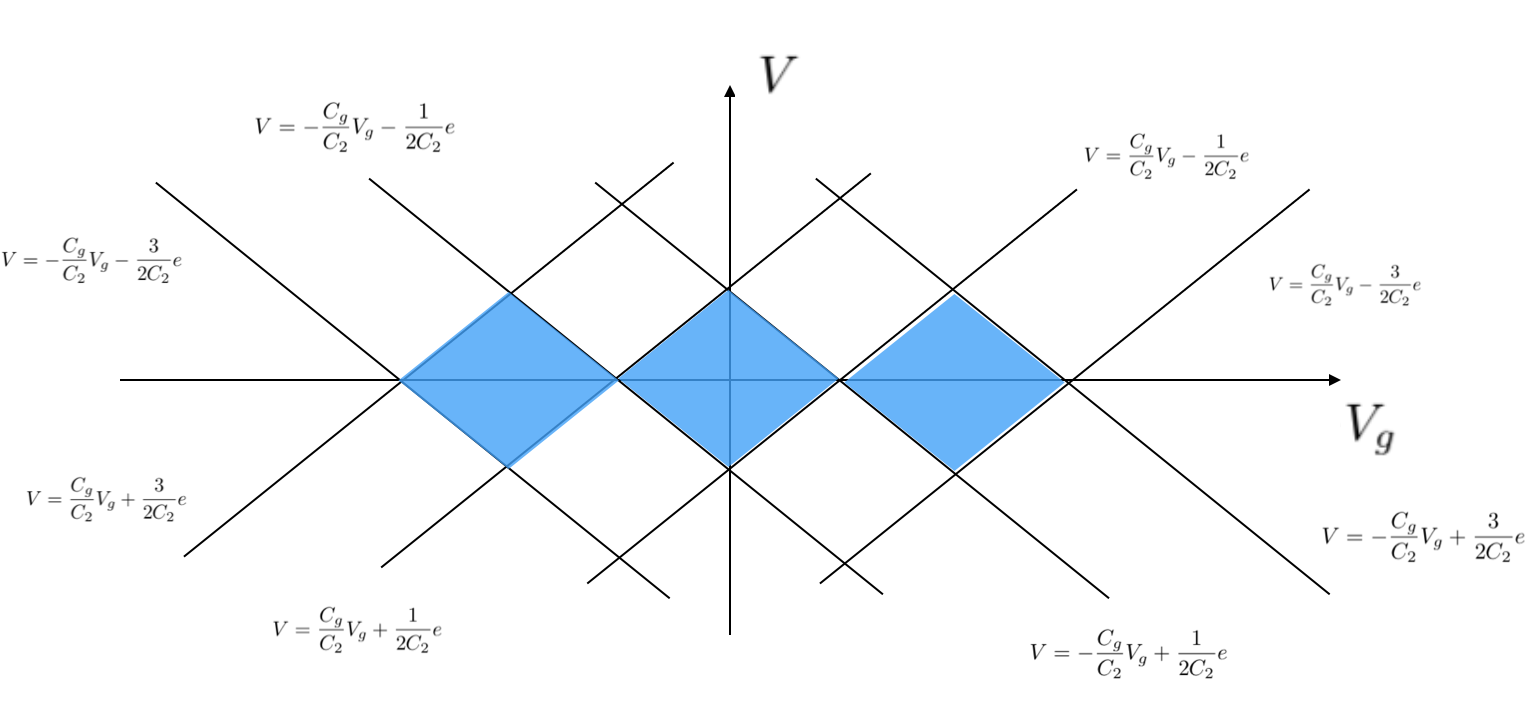
\includegraphics[width=150mm]{coulomb.eps}
  \end{center}
  \caption{$C_1=C_2>>C_g$}
\end{figure}

\begin{figure}[htb]
    \begin{center}
   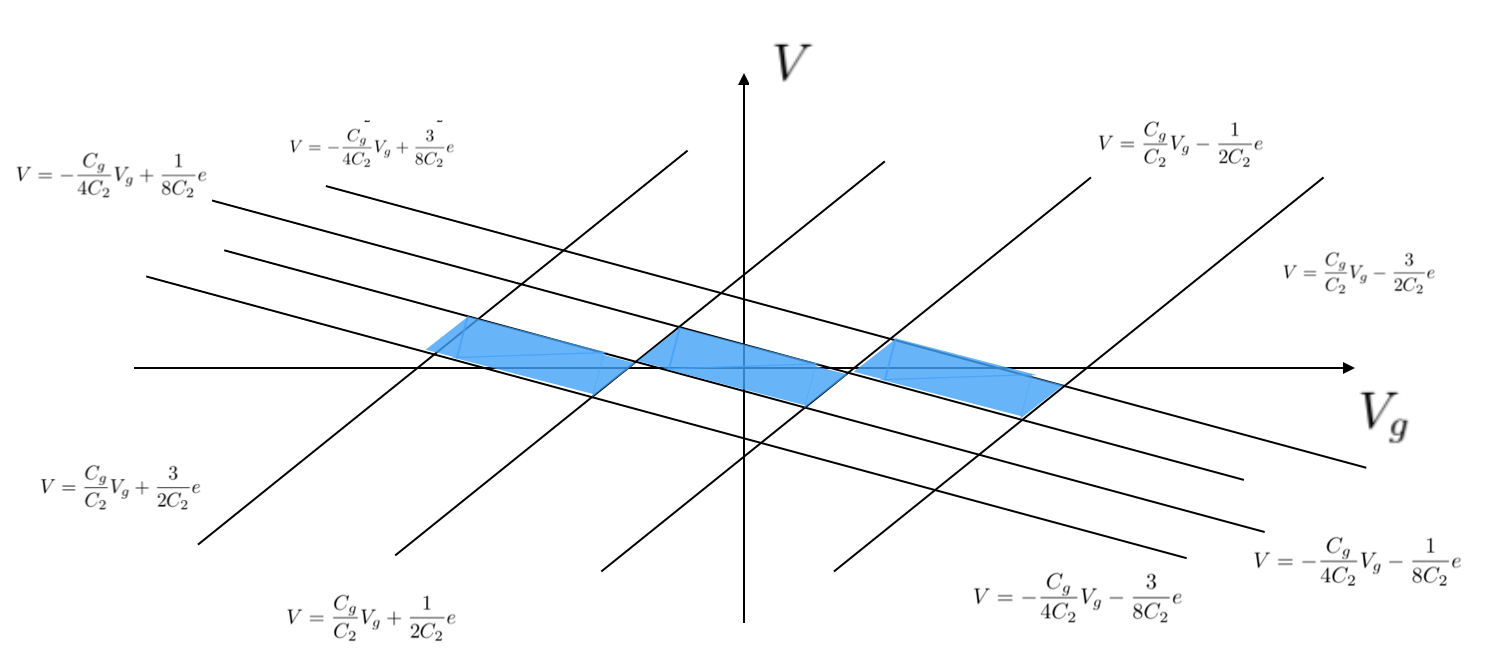
\includegraphics[width=150mm]{coulomb2.eps}
  \end{center}
  \caption{$C_1=4C_2>>C_g$}
\end{figure}


\end{document}